\part{Analyse et implémentations}
\chapter{Détails sur l'implémentation}
\section{Représentation du modèle}
\subsection{Parcours}
Comme expliqué au chapitre précédent un parcours est constitué de plusieurs trajets. Donc la classe {\bfseries Parcours} possédera une liste de trajets. Il regroupe également des informations qui lui sont propres tel qu'un nom et un identifiant. On remarquera également qu'un parcours possède un trajet de référence. Ce trajet est cruciale car il permettra la comparaison avec le trajet qui est effectué. Comme celui-ci pourra être modifié, on le représentera dans la classe {\bfseries Parcours} par son identifiant. On ajoutera à cette classe tout un tas d'attributs servant à déterminer le meilleur temps, la vitesse moyenne, la vitesse maximale sur l'ensemble des trajets effectués.

\subsection{Trajet}
La classe {\bfseries Trajet} représente le chemin qu'un utilisateur emprunte lorsqu'il effectue une course. On y retrouve une liste de points ({\bfseries Location}) nécessaire à la visualisation du trajet ainsi qu'à la comparaison avec le trajet de référence. On gardera également des informations concernant la date à laquelle le trajet a été réalisé ainsi qu'un identifiant pour faciliter le stockage en base. 
\begin{img}
  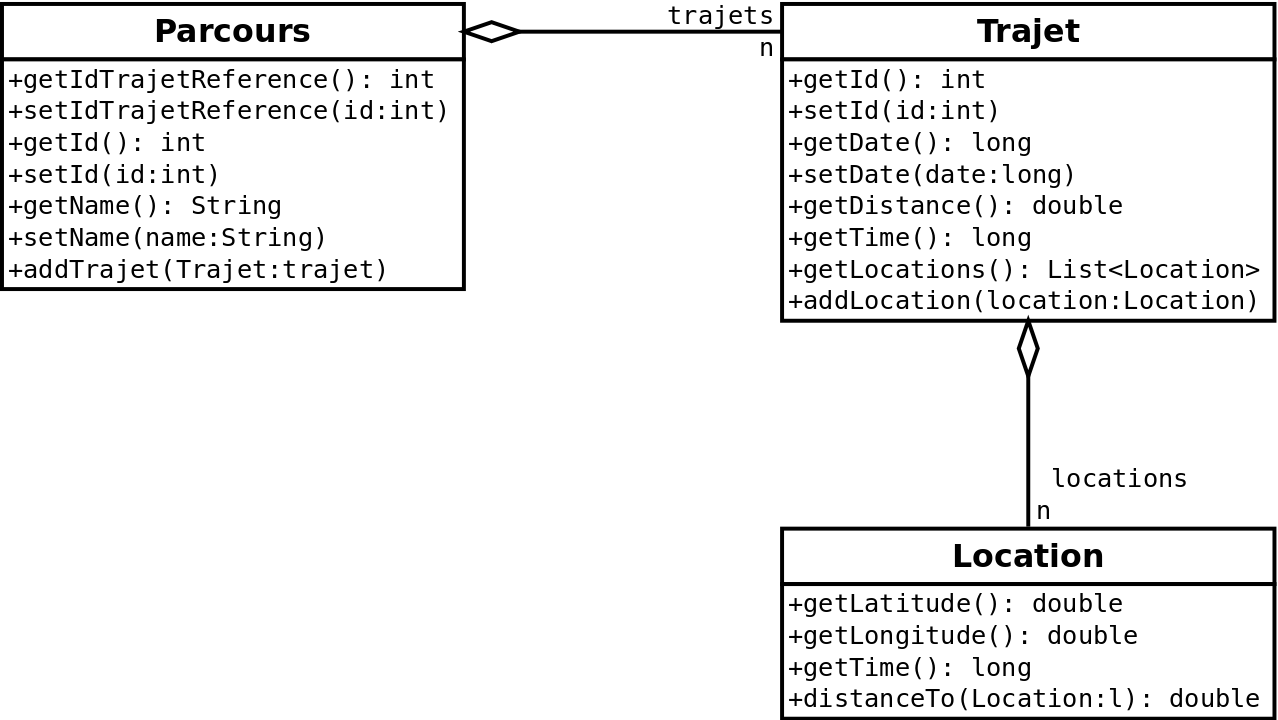
\includegraphics{img/DiagrammeDeClasse.png}
  \caption{Diagramme de classes}
\end{img}